\section{Grundlagen} % (fold)
\label{sec:grundlagen}
In diesem Versuch soll die effektive Masse von Elektronen in Halbleitern
bestimmt werden.
Hierfür wird die Faraday-Rotation von polarisiertem Licht gemessen.
Zunächst werden einige physikalische Grundlagen erläutert, um anschließend
das Messverfahren zu skizzieren und die Ergebnisse darzustellen.

\subsection{Effektive Massen in Halbleitern} % (fold)
\label{sub:effektive_masse}
Halbleiter zeichnen sich durch eine schmale Bandlücke zwischen Leitungs-
und Valenzband aus.
Während die genaue Struktur der Energiebänder komplex ist, reicht meist
eine näherungsweise Betrachtung aus, um physikalische Verhaltensweisen zu
beschreiben.
Hierfür lässt sich die Funktion der Elektronenenergie in Abhängigkeit des
Wellenvektors $\vec{k}$
im Phasenraum $\epsilon(\vec{k})$ als Taylorreihe bis zu einem Term zweiter
Ordnung entwickeln:
\begin{equation}
    \label{eqn:energie}
    \epsilon\left(\vec{k}\right) = \epsilon(0) + \frac{1}{2}\sum_{i=1}^{3}\frac{\partial^2\epsilon}{\partial k_i^2}\cdot k_i^2 + \dots\,.
\end{equation}
Hierbei kann die effektive Masse $m^*$ durch einen Vergleich von
\begin{equation*}
    \epsilon = \frac{\hbar^2 k^2}{2m}
\end{equation*}
mit
\begin{equation}
    m_i^* = \frac{\hbar^2}{\left.\frac{\partial^2\epsilon}{\partial k_i^2}\right|_{k=0}}
\end{equation}
identifiziert werden. Der große Vorteil dieser Betrachtung ist die
Möglichkeit der Behandlung der Elektronen als freie quantenmechanische
Teilchen.
\begin{figure}[h]
    \centering
    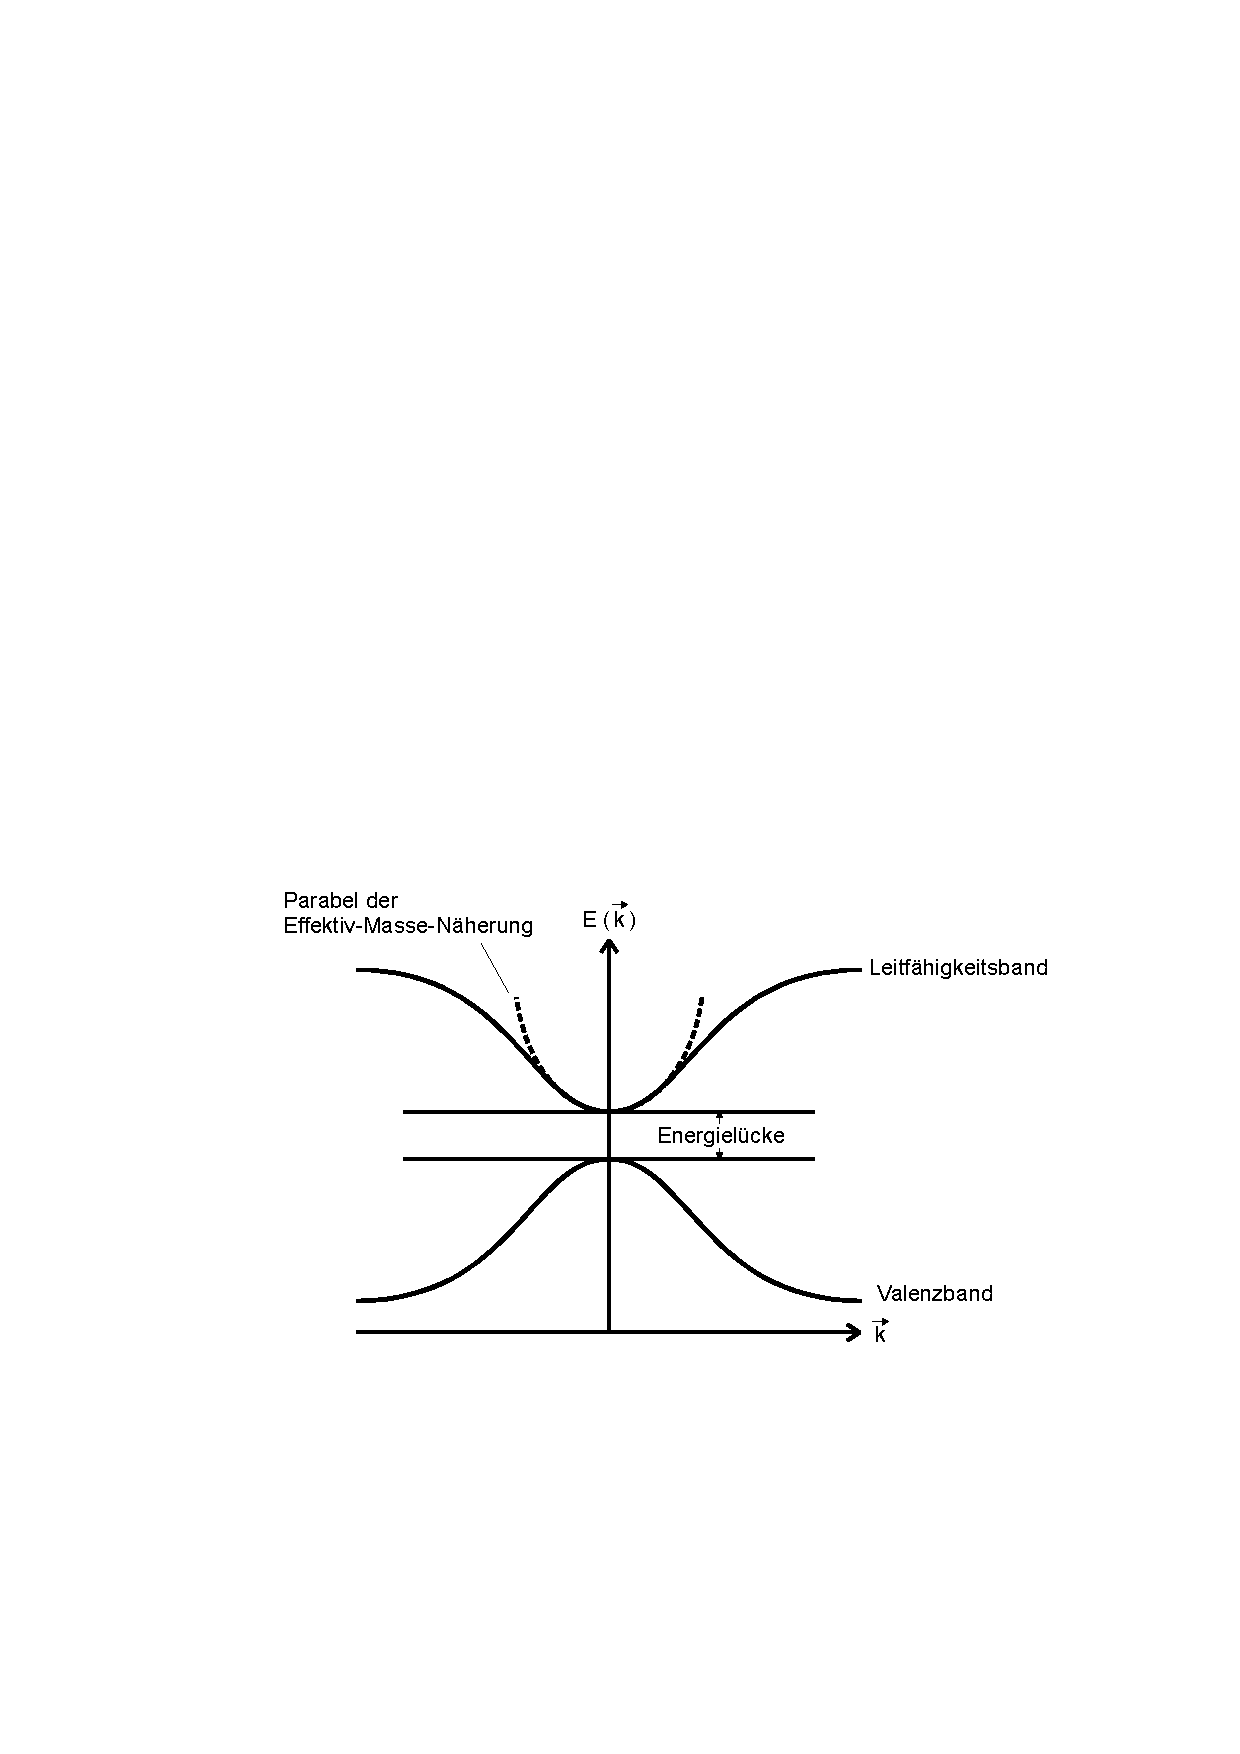
\includegraphics[width=0.8\linewidth]{img/band.pdf}
    \caption{
        Einfache Näherung der Struktur der Energiebänder in einem Halbleiter
        \cite{V46}.
    }
    \label{fig:band}
\end{figure}
In einem symmetrischen Kristall sind die Ausprägungen vom $m_i^*$ in allen
Raumrichtungen identisch und die Funktion \eqref{eqn:energie} lässt sich
vereinfachen zu
\begin{equation}
    \label{eqn:energie_einfach}
    \epsilon\left(\vec{k}\right) = \epsilon(0) + \frac{\hbar^2k^2}{2m^*}\,,
\end{equation}
was den Lösungen der Schrödingergleichung für freie Elektronen entspricht.
Die Notwendigkeit der Betrachtung des periodischen Potentials in einem Kristall
fällt damit weg und der Hamiltonoperator vereinfacht sich zu
\begin{equation*}
    \frac{\hbar^2}{2m_0}\mathrm{\Delta} + V(\vec{r})
    \quad\Rightarrow\quad
    \frac{\hbar^2}{2m^*}\mathrm{\Delta}\,.
\end{equation*}
Für kleine äußere Felder lässt sich das Verhalten der Teilchen sogar
klassisch betrachten und kann durch die Newtonschen Gesetze beschrieben
werden.
% subsection effektive_masse (end)

\subsection{Zirkulare Doppelbrechung} % (fold)
\label{sub:doppelbrechung}
Einige Kristalle haben die Fähigkeit, die Polarisationsebene von linear
polarisiertem Licht zu drehen. Eine Welle $E(z)$, die sich in $z$-Richtung
durch den Kristall ausbreitet hat an der Stelle $L$ im Kristall die Form
\begin{equation}
    \label{eqn:energie_final}
    E(L) = E_0\e^{\i\psi}\left(
        \cos\theta\vec{x_0} + \sin\theta\vec{y_0}
    \right)\,.
\end{equation}
Hierbei wurde die linear polarisierte Welle in einen links- und einen
rechtspolarisierten Anteil mit den jeweiligen Wellenzahlen $k_\text{L}$ und
$k_\text{R}$ zerlegt und es werden die Größen
\begin{align*}
    \psi   &= \frac{L}{2}\left(k_\text{R}+k_\text{L}\right)\\
    \text{und}\qquad\theta &= \frac{L}{2}\left(k_\text{R}-k_\text{L}\right)\\
\end{align*}
eingeführt.
Mit Hilfe der Phasengeschwindigkeit $v_\text{Ph} = \omega/k$, oder dem
Brechungsindex $n=c/v_\text{Ph}$ lässt sich $\theta$ darstellen als:
% Die Größe $\theta$ kann zudem mit Hilfe der Phasengeschwindigkeit
% $v_\text{Ph} = \omega/k$ oder dem Brechungsindex $n=c/v_\text{Ph}$ darstellen,
% wobei die Größen wiederum bezüglich der zirkularen Polarisationsrichtungen
% $R$ und $L$ betrachtet werden:
\begin{equation}
    \label{eqn:theta}
    \theta = \frac{L\omega}{2}
    \left(
        \frac{1}{v_\text{Ph,R}} - \frac{1}{v_\text{Ph,L}}
    \right)
    = \frac{L\omega}{2c}\left(n_\text{R}-n_\text{L}\right)\,.
\end{equation}
Dabei werden die Größen getrennt für die zirkularen Polarisationsrichtungen
$R$ und $L$ für rechts- und links-zirkulares Licht betrachtet.

Im Kristall bilden die Elektronen mit den Atomrümpfen Dipolmomente aus,
die durch die einfallende Lichtwelle angeregt werden und diese weiter
übertragen können.
Insgesamt bildet sich so eine Polarisation $\vec{P}$ des Kristalles aus,
für die mit der Influenzkonstante $\epsilon_0$ und der dielektrischen
Suszeptibilität $\chi$ gilt
\begin{equation}
    \label{eqn:polarisation}
    \vec{P} = \epsilon_0\chi\vec{E}\,.
\end{equation}
In isotropen Materialien entspricht die Suszeptibilität einer skalaren Größe.
Im Allgemeinen ist diese Größe jedoch richtungsabhängig und wird oft
durch einen symmetrischer Tensor beschrieben:
\begin{equation}
    \label{eqn:suszeptibilitaet_inaktiv}
    \mathbf{\chi}_\text{i} =
    \left(\begin{array}{ccc}
        \chi_{xx} & 0 & 0 \\
        0 & \chi_{yy} & 0 \\
        0 & 0 & \chi_{xx} \\
    \end{array}\right)\,.
\end{equation}
Die oben genannte Drehung der Polarisationsebene tritt nun genau dann auf, wenn
die Nebendiagonalelemente $\chi_{xy}$ nicht alle verschwinden, sondern der
Tensor die Gestalt
\begin{equation}
    \label{eqn:suszeptibilitaet_aktiv}
    \mathbf{\chi}_\text{a} =
    \left(\begin{array}{ccc}
        \chi_{xx}    & \i\chi_{xy} & 0 \\
        -\i\chi_{xy} & \chi_{yy}   & 0 \\
        0            & 0           & \chi_{xx} \\
    \end{array}\right)
\end{equation}
annimmt. In diesem Fall treten, wie in der Anleitung \cite{V46} mit Hilfe
des Ansatzes einer ebenen Welle in $z$-Richtung gezeigt, verschiedene
Phasengeschwindigkeiten $v_\text{Ph,R}$, $v_\text{Ph,L}$ für rechts- und
linkspolarisiertes Licht auf.
Für die Größe $\theta$ gilt dann näherungsweise
\begin{equation}
    \label{eqn:theta_cirkular}
    \theta \approx \frac{L\omega}{2c}\frac{1}{\sqrt{1+\chi_{xx}}}\chi_{xy}\,,
\end{equation}
was mit der Phasengeschwindigkeit $v_\text{Ph}$ oder dem Brechungsindex $n$
des Materials auch ausgedrückt werden kann mit
\begin{equation}
    \label{eqn:theta_n}
    \theta
    \approx \frac{L\omega}{2c^2}v_\text{Ph}\chi_{xy}
    = \frac{L\omega}{2cn}\chi_{xy}\,.
\end{equation}
% subsection doppelbrechung (end)

\subsection{Faraday-Effekt} % (fold)
\label{sub:faraday_effekt}
Der Faraday-Effekt beschreibt die Erzeugung doppelt brechender
Eigenschaften eines eigentlich optisch inaktiven Materials mit Hilfe eines
äußeren Magnetfeldes.
In einem Kristall, der sich in einem äußeren Magnetfeld befindet,
findet somit der Übergang
\begin{equation}
\label{eq:inaktiv_to_aktiv}
    \mathbf{\chi}_\text{i} \quad \to \quad \mathbf{\chi}_\text{a}
\end{equation}
statt.
% Ein Kristall, der von einem Suszeptibilitätstensor der Form
% \eqref{eqn:suszeptibilitaet_inaktiv} beschrieben wird gelangt in einem
% Magnetfeld somit zu einer Form wie \eqref{eqn:suszeptibilitaet_aktiv}.
Die im vorigen Abschnitt beschriebenen Dipole aus Elektronen und Atomrümpfen
werden vom einfallenden Licht angeregt und vom äußeren Magnetfeld
in ihrer Bahn beeinflusst.
%
% Dabei werden effektiv die schwingenden Elektronen, die als Dipole vom
% einfallenden Licht angeregt werden, vom äußeren Magenetfeld in ihrer
% Bahn beeinflusst.
Der Polarisationswinkel $\theta$ erfährt dadurch eine Abhängigkeit
von der Magnetfeldstärke $B$ und der Ladungsträgerdichte $N$.
Schließlich kann somit eine Näherung für quasifreie Ladungsträger,
also die Elektronen im Leitungsband aufgestellt werden:
\begin{equation}
    \label{eqn:theta_final}
    \theta_\text{frei}
    \approx \frac{e_0^3}{8\pi^2\epsilon_0 c^3}
    \frac{1}{m^2}\lambda^2 \frac{NBL}{n}\,.
\end{equation}
Hierbei tauchen die Elementarladung $e_0$ und die Wellenlänge $\lambda$ des
einfallenden Lichtes auf.

% subsection faraday_effekt (end)
% section grundlagen (end)
\clearpage
\section{Messung des Polarisationswinkels $\theta$} % (fold)
\label{sec:messung}
In der hier durchgeführten Messung kann die Masse $m$ in der oben genannten
Gleichung \eqref{eqn:theta_final} mit der effektiven Masse $m^*$ der
Elektronen identifiziert werden.
Somit ermöglicht die Bestimmung des Polarisationswinkels $\theta$ eine Messung
der effektiven Masse $m^*$.

\begin{figure}[h]
    \centering
    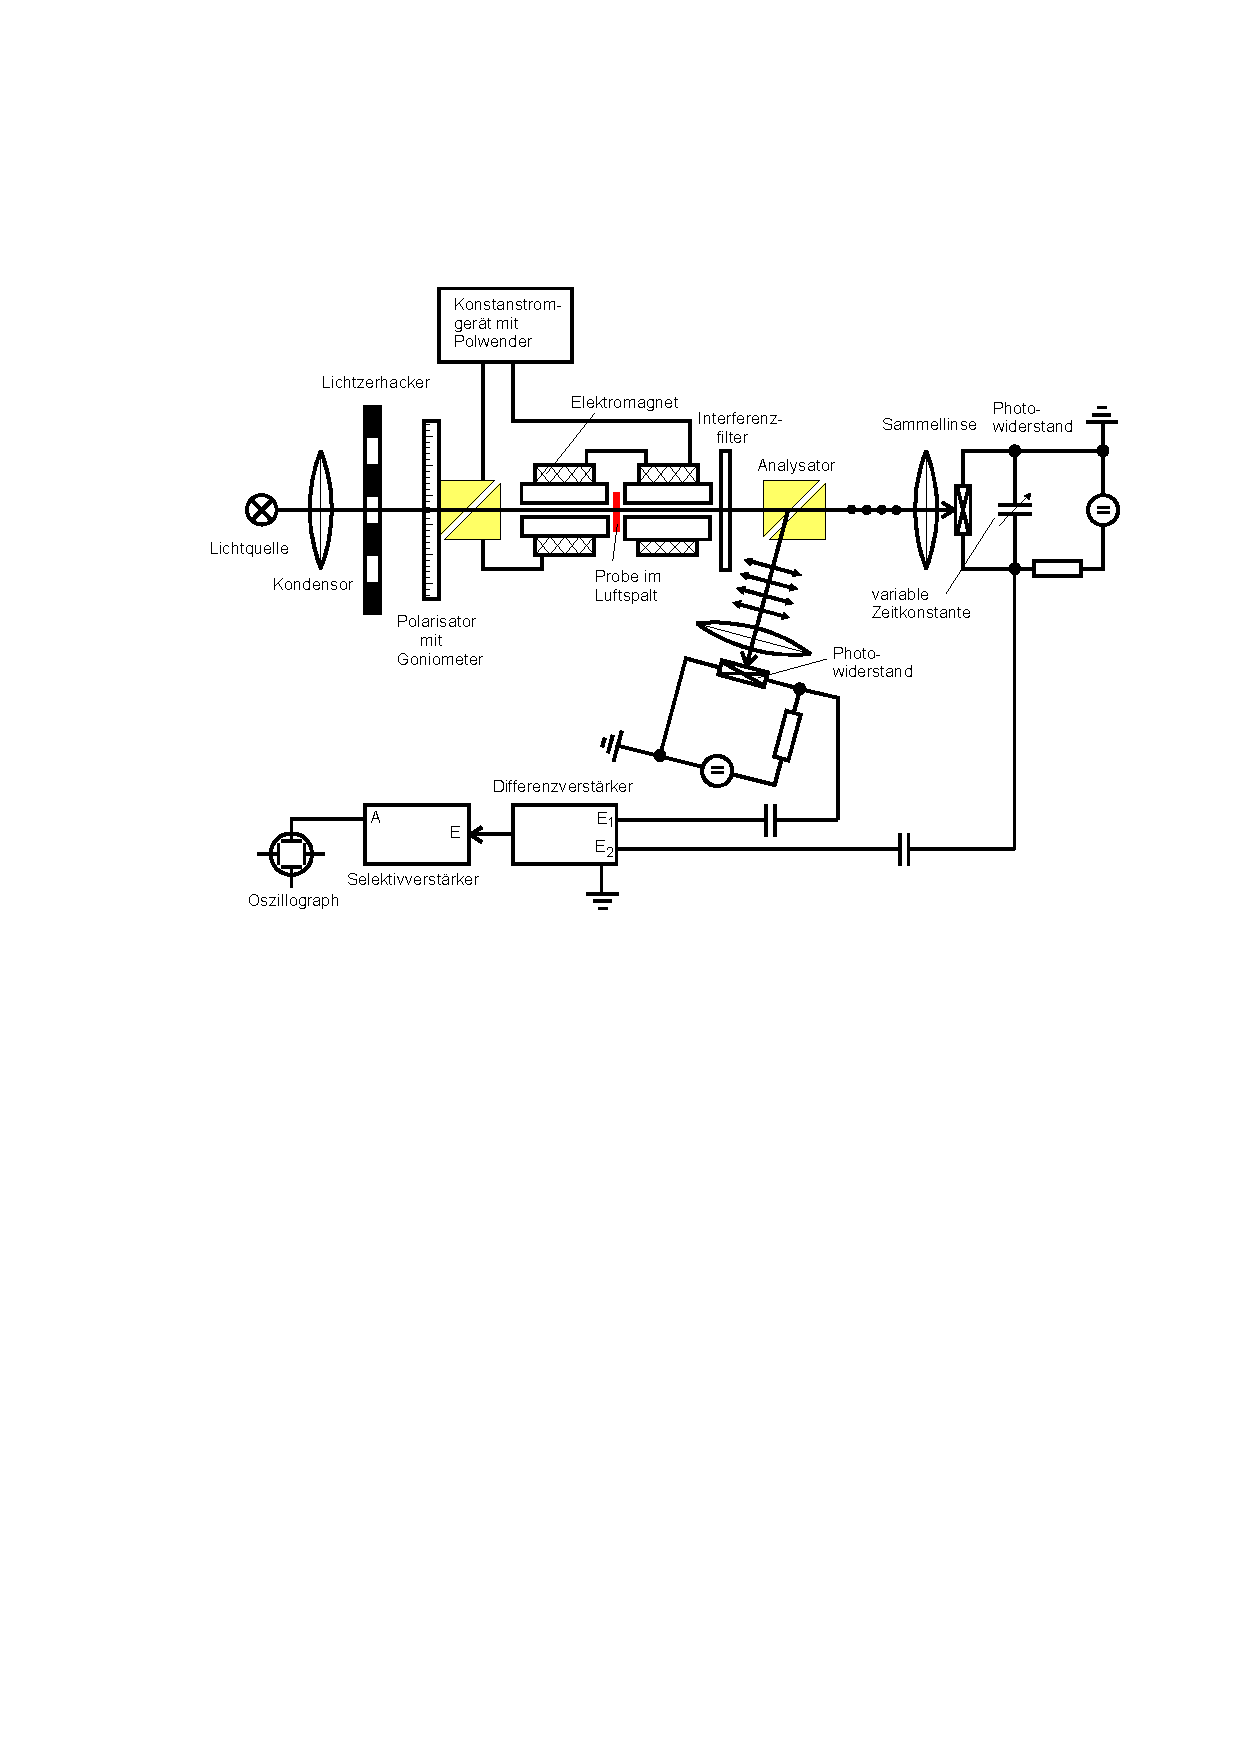
\includegraphics[width=0.9\linewidth]{img/aufbau.pdf}
    \caption{
        Schematische Darstellung der Messapparatur \cite{V46}.
    }
    \label{fig:aufbau}
\end{figure}
Der Versuchsaufbau ist in Abbildung \ref{fig:aufbau} schematisch dargestellt.
Der zu untersuchende Halbleiterkristall kann in einen Elektromagneten
eingebracht werden,
dessen Magnetfeldrichtung umpolbar ist, um den Winkel $\theta$
effektiv verdoppeln zu können.
Als Lichtquelle dient eine Halogen-Lampe, die überwiegend infrarotes Licht
emittiert.
Ein Lichtzerhacker, der hinter der Lampe angebracht ist und mit einem
Selektivverstärker gekoppelt wird, ermöglicht eine effektive
Rauschunterdrückung.
Das Licht wird zunächst mit einem Glan-Thompson-Prisma polarisiert, welches
durch ein Goniometer gedreht werden kann.
Anschließend durchleuchtet der Lichtstrahl die Probe.
Das Licht wird hinter der Probe durch ein weiteres Glan-Thompson-Prisma in
zwei, senkrecht zueinander stehende Polarisationsebenen aufgeteilt, deren
Intensität jeweils mittels Photowiderständen in ein Spannungssignal
umgewandelt wird.
Ein Differenzverstärker gibt schließlich das Differenzsignal der
Photospannungen auf ein Oszilloskop, dessen Amplitude dann proportional zur
Drehung der Polarisationsebene des ausfallenden Lichtes ist.

Zur Justage der Apparatur muss zunächst geprüft werden, ob das Signal ohne
eingelegte Probe und ohne eingeschaltetes Magnetfeld auf Null sinkt.
Anschließend, kann eine Probe in den Elektromagneten eingebracht und
das Magnetfeld eingeschaltet werden.
Die Polarisationsrichtung des Lichts aus dem ersten Glan-Thompson-Prisma wird
nun in der Probe gedreht, wodurch die Signalspannung steigt.
Durch Einstellen des maximalen Signals bei beiden Magnetfeldrichtungen
lässt sich anschließend der Rotationswinkel $\theta$ bestimmen:
\begin{equation}
    \label{eqn:theta_messung}
    \theta = \frac{1}{2}\left(\theta_1-\theta_2\right)\,.
\end{equation}
Hierbei bezeichnen $\theta_1$ und $\theta_2$ die beiden Stellungen des ersten
Glan-Thompson-Prismas.

% section messung (end)
